\documentclass[border=10pt]{standalone}
\usepackage{tikz}
\usetikzlibrary{decorations.pathmorphing, patterns}

\begin{document}

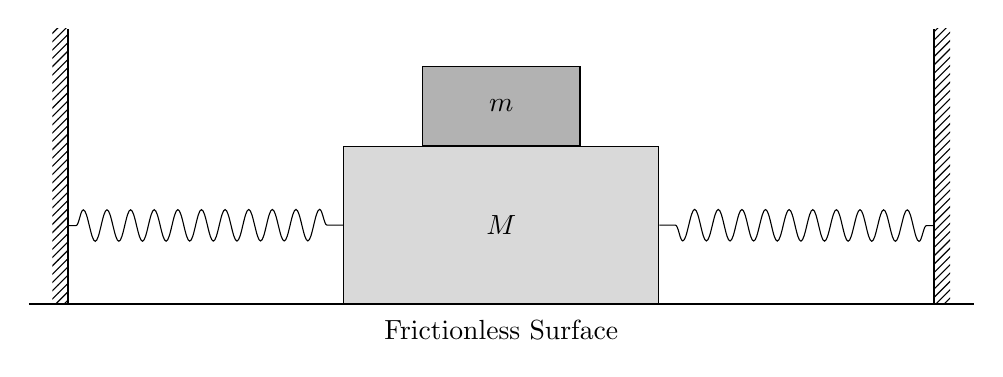
\begin{tikzpicture}

% --- Define reusable styles and key coordinates ---
\tikzset{
    spring/.style={
        decorate,
        decoration={snake, amplitude=2mm, segment length=3mm, post length=1mm, pre length=1mm}
    }
}
% Define the vertical level for the ground and the center of the mass
\def\groundlevel{0}
\def\massheight{2}
\def\springlevel{\groundlevel + \massheight/2} % This ensures springs are at the mass's vertical center

% 1. Draw the frictionless surface
\draw[thick] (-6, \groundlevel) -- (6, \groundlevel) node[pos=0.5, below=2pt] {Frictionless Surface};

% 2. Draw the vertical walls
\draw[thick] (-5.5, \groundlevel) -- (-5.5, 3.5);
\fill[pattern=north east lines] (-5.7, \groundlevel) rectangle (-5.5, 3.5);

\draw[thick] (5.5, \groundlevel) -- (5.5, 3.5);
\fill[pattern=north east lines] (5.5, \groundlevel) rectangle (5.7, 3.5);

% 3. Draw the larger rectangular mass block
\node[draw, fill=gray!30, minimum width=4cm, minimum height=\massheight cm, anchor=south] (large_mass) at (0, \groundlevel) {$M$};

% 4. Draw the left spring (now perfectly horizontal)
\draw[spring] (-5.5, \springlevel) -- (large_mass.west);

% 5. Draw the right spring (now perfectly horizontal)
\draw[spring] (5.5, \springlevel) -- (large_mass.east);

% 6. Draw the smaller mass resting on the first mass
\node[draw, fill=gray!60, minimum width=2cm, minimum height=1cm, anchor=south] (small_mass) at (large_mass.north) {$m$};

\end{tikzpicture}

\end{document}